\documentclass[conference]{IEEEtran}
% This is stripped down to basically the ieee bare_conf.tex header
\usepackage{amssymb,amsmath}
% use upquote if available, for straight quotes in verbatim environments
\IfFileExists{upquote.sty}{\usepackage{upquote}}{}
% use microtype if available
\IfFileExists{microtype.sty}{%
\usepackage{microtype}
\UseMicrotypeSet[protrusion]{basicmath} % disable protrusion for tt fonts
}{}
\usepackage{hyperref}
\PassOptionsToPackage{usenames,dvipsnames}{color} % color is loaded by hyperref
\hypersetup{unicode=true,
            pdftitle={Identifying the True Origin of DNS Traffic Without Reference to Client Source Address},
            pdfborder={0 0 0},
            breaklinks=true}
\urlstyle{same}  % don't use monospace font for urls
% -- biblio. set natbib: true in pandoc for silly hacks around pandoc \cite{} vs \citep{}
\usepackage{cite}
\bibliographystyle{IEEEtran}
\let\citep\cite
% if you want the [2, 3] vs IEEE [2], [3]
\renewcommand{\citepunct}{,\penalty\citepunctpenalty\ }

\title{Identifying the True Origin of DNS Traffic Without Reference to Client
Source Address}
% author names and affiliations
% use a multiple column layout for up to three different
% affiliations
\author{\IEEEauthorblockN{Joe Abley}\IEEEauthorblockA{Western University, London, Ontario, Canada \\ Afilias Canada, Toronto, Ontario, Canada \\ \href{mailto:jabley@uwo.ca}{\nolinkurl{jabley@uwo.ca}},
\href{mailto:jabley@afilias.info}{\nolinkurl{jabley@afilias.info}}}}





\date{2018-12-05 22:37:08 -0500}
\setlength{\parindent}{0pt}
\setlength{\parskip}{6pt plus 2pt minus 1pt}
\let\tightlist\relax % silly pandoc thing

% --- user includes
% Put your preamble here. Example.
% subfigures
\usepackage{subfig}
% dots in filenames
\usepackage{graphicx, grffile}
% bold math
\usepackage{bm}
% colours
\usepackage[usenames,dvipsnames]{xcolor}
% suppress month in bibliography
%\AtEveryBibitem{\clearfield{month}}
%\AtEveryCitekey{\clearfield{month}}

% texdef -t latex -f {cmdname} to see if cmd is already defined

% Letters in fancy font (expectation, integers, reals, normal dist)
\newcommand{\E}[1]{\operatorname{\mathbb{E}}{\left[#1\right]}}
\newcommand{\Z}{\mathbb{Z}}
\newcommand{\R}{\mathbb{R}}
\newcommand{\N}{\mathcal{N}}

\begin{document}
\maketitle
\begin{abstract}
We demonstrate a model that is able to classify the originating system
respobsible for stateless Domain Name System (DNS) traffic received at
an authoritative DNS server without reference to source address. The
ability to determine whether particular DNS query traffic received at an
authoritative server is legitimately sourced from a particular client
system is useful in identifying various classes of malicious traffic in
production DNS systems.
\end{abstract}

\section{Introduction}\label{sec:introduction}

\label{sec:introduction}

The Domain Name System (DNS) includes a wire protocol with which
structured requests and responses are exchanged over a network. The DNS
protocol was originally specified \citep{rfc1034}\citep{rfc1035} for use
over both the Transmission Control Protocol (TCP) \citep{rfc793} and the
User Datagram Protocol (UDP) \citep{rfc768} and the use of other
transports have also been documented
\citep{rfc7858}\citep{rfc8484}\citep{huitema-quic-dnsoquic-05}. At
present, however, UDP is the overwhelmingly dominant transport protocol
in use; for example, according to statistics published by ICANN for
queries received at the L root server, UDP accounts for 98\% of all
queries
received\footnote{\url{http://stats.dns.icann.org/plotcache/L-Root/transport_vs_qtype/2018-12-03T00:00-2018-12-03T23:59-all.html}}.

Since UDP transport for DNS is stateless, consisting of single-datagram
queries and responses with no setup or tear-down handshake, there are
limited opportunities to verify the legitimacy of a source address. DNS
servers are consequently frequently used as amplifiers in reflection
attacks \citep{rfc5358}. Although some such attacks are trivially
identified, e.g.~by Query Type (QTYPE), many are more difficult. By
choosing query parameters that match legitimate, real-world use of the
DNS, attackers can make it difficult for their traffic to be identified
and blocked without causing collateral damage. This is especially true
of amplification attacks against DNS resolvers.

The clients of authoritative DNS servers are most usually DNS resolvers.
These client systems receive requests from end-user applications (or
downstream resolvers). Different client resolver systems are observed to
send different mixes of DNS traffic; for example, a resolver system that
mainly serves end-users will send a different mixture of queries to
authoritative servers than one which serves a specific application like
Internet mail \citep{rfc5321}, which might reasonably be expected to
have a much higher proportion of query traffic with \texttt{QTYPE=MX}.

Afilias Canada\footnote{\url{https://afilias.info/}} operates
authoritative DNS infrastructure for around 300 top-level domains,
including several that attract high levels of query traffic such as INFO
and ORG. This infrastructure is distributed globally using anycast
service distribution \citep{rfc4786}, using commodity transit services,
public peering and so-called Private Network Interconnects (PNIs). The
real origin of queries received over a PNI can be known with high
accuracy; the origin of queries received over the Internet, in contrast,
cannot. We refer to the former as \emph{trusted} paths, and the latter
as \emph{untrusted}. Trusted paths exist to Google Public
DNS\footnote{\url{https://dns.google.com}}, a public DNS resolver system
configured for use by a large number of end-users, and
Facebook\footnote{\url{https://www.facebook.com}}, whose resolver
systems are mainly used by back-end systems that build previews for
links shared between users of Facebook's social media platform. The
traffic patterns of each are expected to be usefully different.

While real-time anomoly detection in DNS traffic remains an elusive
problem, the ability to classify traffic apparently received by
particular sources as being legitimate is useful in the forensic
analysis of traffic spikes since it provides the opportunity to
distinguish between illegitimate, unwanted traffic and traffic from
clients that just happen to be busy, e.g.~due to a burst in popularity
in a particular web page, or changes in the Time To Live (TTL)
parameters of high-use domain names. This paper describes a system that
aims to provide such a classification.

A raw DNS dataset is collected in the form of individual (request,
response) DNS messages received from and sent to a single apparent
source over period of two weeks. We split the resulting query stream
into five minute intervals and from each we extract a vector of
variables that describes the traffic received from each client during
that time. Each such vector, once normalised, represents a single
observation related to a single client. Observations that correspond to
traffic received from trusted sources can be used as a training dataset.
Observations corresponding to DNS traffic that definitively did not
arrive from a trusted source can also be incorporated as ``other''. The
resulting model can be used to classify five-minute samples of query
streams from purported single sources to classify the origin of the
query traffic as ``Facebook'', ``Google'' or ``Other''. Since query
sources for each category feature in an equal number of traffic samples,
it is straightforward to produce a training dataset that is balanced
across the three categories.

This paper is organised as follows. Section \ref{sec:introduction}
introduces the problem and provides some high-level background on the
DNS. Section \ref{sec:background} provides a short introduction to the
algorithms and accuracy measures that are used to build the model. Some
other work on applying machine learning techniques to problems in the
DNS are described in section \ref{sec:related}. Data collection and
preprocessing, feature engineering and choice of learning and validation
algorithms are discussed in section \ref{sec:methodology}. Section
\ref{sec:evaluation} describes the evaluation of the resulting model.
Section \ref{sec:conclusion} provides a summary of the work described in
this paper, and section \ref{sec:future} identifies some areas for
future study.

\section{Background}\label{sec:background}

\label{sec:background}

Two multiclass classifiers are evaluated for this model in section
\ref{sec:classifiers}, below. The approach used to evaluate the accuracy
of each is described in section \ref{sec:accuracy}. These models are
used to classify features of individual five-minute samples of DNS
reponse data according to source system by treating each sample as a
single observation. A brief discussion of other approaches that might
usefully consider each sample as a point along a time series can be
found in section \ref{sec:future}.

\subsection{Classifier Models}\label{sec:classifier-models}

\label{sec:classifiers}

We consider both Support Vector Machine and Random Forest models and
select the most successful one based on 10-fold validation.

\subsubsection{Multiclass Support Vector
Machine}\label{sec:multiclass-support-vector-machine}

\label{sec:svmmethod}

The classifier used in this paper was constructed as a series of Support
Vector Machines (SVM), each used as a binary classifier. SVM represents
\(n\)-dimensional support vectors in an \(n\)-axis hyperspace and
identifies a hyperplane boundary between observations known to be in
different categories to facilitate classification of unlabelled test
sets. Those boundaries can then be used to classify unlabelled
observations.

Multiclass classification is achieved using \(k(k-1)/2\)
\emph{one-against-one} binary classifiers combined with a max-wins
voting scheme, as discussed in \citep{10.1007/11494683_28}.

The SVM implementation used to construct this model exposes several
hyperparameters that can be tuned, as well as a native grid search to
assist identification of optimal parameters for a supplied validation
dataset.

\subsubsection{Random Forest}\label{sec:random-forest}

\label{sec:rfmethod}

Random Forests (RF) \citep{Breiman2001} combine many decision trees at
training time into an ensemble learning model. RF uses bootstrap samples
to introduce a random component into the tree-building process, whilst
also reducing correlation amongst trees, adding noise to perturb the
tree structure and using a random subset of available predictors each
each split. Each of \(m\) models in the resulting ensemble is used to
generate a prediction for a new sample and those predictions are
averaged to give the prediction from the entire forest.

The tuning parameters for the RF ensemble model are:

\begin{itemize}
\tightlist
\item
  the size of the subset of predictors randomly selected at each split,
  \(m_try\). Breiman suggests setting \(m_try\) to be one third of the
  number of predictors.
\item
  the number of trees in the forest. Breiman has proved that random
  forests are immune from overfitting, but the accuracy
  benefit:computational cost is expected to decrease as the forest
  becomes larger.
\end{itemize}

\subsection{Accuracy Measures}\label{sec:accuracy-measures}

We calculate a confusion matrix over a test dataset:

\begin{center}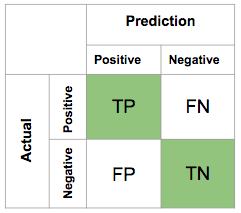
\includegraphics[width=0.5\linewidth]{confusion_matrix} \end{center}

Since we intend to ensure that we have a balanced dataset between the
three classifications of traffic samples, we are able to use a
straightforward measure of accuracy, A:

\[A = \frac{TP + TN}{TP + FP + TN + FN}\]

Without a particular application for the models, it is difficult to
assess the relative importance of false positives or false negatives in
our model. However, as a kindness to a reader with a business case in
mind, we calculate the precision, P, the recall, R and the specificity,
S:

\[P = \frac{TP}{TP + FP}\]

\[R = \frac{TP}{TP + FN}\]

\[S = \frac{TN}{TN + FP}\]

As is conventional, we also calculate the F1 score, F, as the harmonic
mean of the precision and recall metrics:

\[F = \frac{2PR}{P + R}\]

\section{Related Work}\label{sec:related-work}

\label{sec:related}

Machine learning techniques were applied to the problem of classifying
so-called core domains as part of a threat assessment in a production
system at
Nominum\footnote{Nominum was acquired by Akamai in November 2017}
\citep{Yuzifovichbotconf2017} \citep{YuzifovichOARC2017}. This problem
has some similarities to the problem described in this paper, and
illustrates the use of continuous learning to upadate an already-trained
model on arrival of new data.

The .NZ registry maintains a set of business intelligence datasets which
are constructed in part by analysis of queries received at authoritative
DNS servers. In order to improve the accuracy of those datasets, machine
learning techniques were used to build models that could classify query
sources as DNS resolvers or other systems (e.g.~systems performing
active monitoring of the DNS). The work included extensive feature
analysis and incorporated substantial domain knowledge derived from
earlier analysis. \citep{Qiao2018} \citep{QiaoOARC2018}.

A study in the application of different machine learning techniques was
presented in \citep{Sammour2017} as part of an attempt to train a model
to identify Internet traffic tunnelled over the DNS protocol.

The approach described in this paper differs from other approaches
described above in that it acknowledges the problems inherent in
grouping DNS transactions together without the ability to be certain
that the apparent sources of DNS queries are legitimate.

\section{Methodology}\label{sec:methodology}

\label{sec:methodology}

\subsection{Overview}\label{sec:overview}

\label{sec:methodology_overview} A complete set of DNS query data
received with UDP transport over trusted and untrusted paths at a major
anycast site in Ashburn, VA, USA was collected. This source data is
based on raw packet captures in PCAP
format\footnote{PCAP, named after the C library \texttt{libpcap}, is the file format used by the \texttt{tcpdump} utility},
post-processed into \emph{dnscount} objects to extract various
parameters from the raw DNS messages: a timestamp; client and server
adresses (IPv4 and IPv6); the query type; query name; transport
protocol; response code and DNS message flags. Separate \emph{dnscount}
objects are stored for queries and responses; the query objects differ
slightly in composition since they naturally do not include a response
code.

The \emph{dnscount} objects are centralised using
Redis\footnote{\url{https://redis.io/}} message brokers for integration
in other Afilias traffic measurement systems. Since the response objects
contain a superset of the information contained within the query objects
(they include a response code), and since they represent the results of
queries that are known to be well-formed to the extent that a nameserver
can produce a response, only the response objects for a sample period
were extracted for use in training this model. The production Redis
message brokers were not used since doing so would involve a release
engineering process which would introduce unnecessary cost and delay to
the collection process.

\subsection{Data Reduction}\label{sec:data-reduction}

Query summaries at just this site represent around 500GB of data when
compressed using bzip2\footnote{\url{http://www.bzip.org/}}, and hence
an in-place reduction and summarisation process was undertaken:

\begin{enumerate}
\def\labelenumi{\arabic{enumi}.}
\tightlist
\item
  Only data from the first two weeks in November 2018 were considered.
  This seems intuitively like a long enough period to accommodate
  different workday and weekend behaviour without represending an
  unmaageable data set, although it seems intuitively true that a longer
  sample period would result in a better model (see also section
  \ref{sec:future});
\item
  Query \emph{dnscount} objects were discarded, since the corresponding
  response objects contain a superset (see section
  \ref{sec:methodology_overview});
\item
  Response objects with TCP transport were discarded, since transactions
  over an established TCP session have authenticated endpoint addresses
  through the TCP setup handshake;
\item
  Collections of the remaining objects within five-minute sample buckets
  were used to produce a set of summary observations for each (site,
  client, bucket), as described in section \ref{sec:datasetextraction}.
\end{enumerate}

The resulting summaries (compressed again using bzip2) occupied around
5GB, which is a more manageable data volume for transport over a network
to a central location. This data also contains no query names, allowing
greater confidence that it contains no personally-identifiable
information and hence presents no significant threat to personal
privacy.

\subsection{Data Extraction}\label{sec:data-extraction}

\label{sec:datasetextraction}

Individual \emph{dnscount} records were summarised in five-minute
intervals in order to characterise the nature of DNS traffic for the
corresponding (\emph{timestamp}, \emph{sitecode}, \emph{client}). The
resulting observations for each contained the following variables. These
were selected based on general domain knowledge about the DNS and about
the nature of the end-systems that trigger DNS queries to be sent from
Google and Facebook resolvers.

\begin{itemize}
\tightlist
\item
  (\emph{timestamp}, \emph{sitecode}, \emph{client})
\item
  number of responses counted in each five-minute sample interval
\item
  length of the largest observed label in all query name
\item
  the mean length of all observed labels in all query names
\item
  the number of unique top-level labels observed in all query names
\item
  the number of unique second-level domains observed in all query names
\item
  the proportion of query names that consisted of 1, 2, 3 or 4 labels
  (exposed as four separate variables)
\item
  the proportion of responses with response
  code\footnote{\url{https://www.iana.org/assignments/dns-parameters/dns-parameters.xhtml\#dns-parameters-6}}
  0, 1, 2, 3, 4 5, 6, 7, 8, 9 or 10 (eleven separate variables)
\item
  the proportion of responses with query
  type\footnote{\url{https://www.iana.org/assignments/dns-parameters/dns-parameters.xhtml\#dns-parameters-4}}
  1, 2, 5, 6, 15, 16, 28, 48 and 255 (eight separate variables)
\end{itemize}

Closer examination of this summary set revealed data for around two
million clients; of those two million, 80\% of responses observed during
the sample window were sent to just ten thousand. This is a decidedly
asymmetric distribution with a long tail.

Training and validation datasets were extracted from these summary sets
by collecting all observations for (\emph{t}, \emph{sitecode},
\emph{client}) \(\forall t\), \emph{sitecode} = IAD1 and each of:

\begin{enumerate}
\def\labelenumi{\arabic{enumi}.}
\tightlist
\item
  \emph{client} is known to be reachable via the Google PNI (candidate
  Google dataset);
\item
  \emph{client} is known to be reachable via the Facebook PNI (candidate
  Facebook dataset);
\item
  \emph{client} is not reachable via any PNI (candidate ``other''
  dataset).
\end{enumerate}

\emph{Describe the resulting datasets}

\subsection{Feature Engineering}\label{sec:feature-engineering}

\begin{itemize}
\tightlist
\item
  derive day-of-week and hour-of-day from date field; discard month and
  year since they would be the same for all observations
\item
  discard site code, since it's the same for all observations
\end{itemize}

\subsection{Validation Process}\label{sec:validation-process}

We validate each model described in section \ref{sec:classifiers} using
k-fold cross-validation over the training dataset with \(k=10\). This
provides an assessment of each model through ten folds of the source
data, giving a better measure of validation than a single
training/validation split.

The selected model is then trained over the entire training set, and
applied to untrained data to measure its accuracy.

\section{Evaluation}\label{sec:evaluation}

\label{sec:evaluation}

Results of the process I applied

Can include a paragraph describing what languages, packages and
libraries were used.

Possibilities: accuracy measures, graphs showing tuning process, tables
and graphs comparing different approaches, tuned parameter ranges and
selected values.

No code.

\section{Conclusion}\label{sec:conclusion}

\label{sec:conclusion}

Short summary of the paper/report

Should include problem description, how I solved it and the main
results.

\section{Future Study}\label{sec:future-study}

\label{sec:future}

\begin{itemize}
\tightlist
\item
  different algorithms
\item
  incorporate new classes (new trusted paths to resolvers)
\item
  string-similarity metrics for QNAMEs
\item
  quantitative measurements of query entropy
\item
  larger sample period
\item
  continuous learning model
\item
  recurrant neural networks or other models that exhibit temporal
  dynamic behaviour for a time sequence
\end{itemize}

It is reasonable to expect that the grouping and ordering of DNS queries
might be relevant in the classification of a query stream as originating
from a particular DNS resolver. For example, the DNS Security Extensions
(DNSSEC) specification\cite{rfc4033} accommodates flexibility in the
order in which DNSSEC resource record sets are retrieved when a resolver
with an empty cache performs validation on an answer from a signed zone;
certain
applications\footnote{For example, qmail sends queries with QTYPE=ANY in an attempt to accelerate the process of retrieving answers that otherwise would require separate queries with QTYPE=A, AAAA and MX. The rarity of this approach was exposed when support for ANY queries on the server side started to become constrained. See \url{https://fanf.livejournal.com/122220.html} for related commentary.}
are also known to exhibit specific behaviour when using the DNS, and
resolvers that serve a community of such applications might exhibit
corresponding identifying behaviour. Particular web services use
signature combinations of content distribution network or embedded
advertiser beacons that might well provide a useful signature through a
resolver, even with the significant caching potential of answers
obtained from top-level domain authoritative nameservers.

The models described in this paper treat each query stream as an
unordered set of observations. The applicability of other models whose
training can be influenced by the ordering of data, e.g.~those based on
recurant multilayer perceptron networks, seem worthy of future
investigation.

\section{Colophon}\label{sec:colophon}

This document has been written in R
Markdown\footnote{\url{https://rmarkdown.rstudio.com}}; the code used to
produce the output included in this document is consequently included
with the document
source\footnote{\url{https://github.com/ableyjoe/uwo-mesc/tree/master/ECE-9603A-001-GF18/project}}.
The production of this document in IEEEtran style from R Markdown was
informed by a pseudonomymously-attributed community
project\footnote{\url{https://github.com/mathematicalcoffee/IEEEtran-rmarkdown}}.

\bibliography{IEEEabrv,./project}

\end{document}
